\chapter{Analysis Optimization}\label{sec:analysis_optimization}
\red{or should this chapter be called multivariate discriminants}

After selecting objects that represent the final state of the physical process under investigation, a metric needs to be constructed sensitive to the result of a hypothesis test which assesses the realization of this process in nature. Often, this metric takes the form of a kinematic variable, such as the invariant mass of the Higgs pair system $m_\text{HH}$ in this analysis, designed to differentiate between signal and background events. As elaborated in Chapter \ref{sec:statistics}, the underlying statistical test employs frequentist principles, thus histograms derived from this metric serve as inputs to these tests. Throughout the development of this variable, various optimizations typically aim to maximize the signal-to-background ratio as a proxy for the statistical tests expressivity.

Since the purpose of this quantity is to separate signal from background it is well suited to be anaylized with a \ac{ml} model. While such models have gained widespread usage in particle physics \citep{albertsson2019machine,shlomi2020graph,feickert2021living,Schwartz2021Modern}, their effectiveness is limited when they are only optimized for signal-to-background discrimination. This is because their training does not usually consider broader goals like assessing discovery significance or establishing confidence levels.

The signal-to-background ratio or the efficacy of a \ac{ml} model in separating events correlates to some extent with the performance of the statistical test.  However, this relationship often remains suboptimal because uncertainties, which can significantly influence the outcome of hypothesis tests, are not typically considered during the training phase of \ac{ml} models.

To address these challenges, \textit{\ac{neos}} \citep{Simpson_2023} offers a promising solution. This approach incorporates the statistical model and its uncertainties into the \ac{ml} model's training process, aligning it more closely with the primary goal of determining whether a new process exists. This chapter provides a brief introduction to machine learning and explains the \textit{\ac{neos}} approach and its application in this analysis in detail.

\section{Machine Learning}
\ac{ml} refers to algorithms that enable computers to learn from data to make predictions for some specific task without being explicitly programmed for \citep{kubat2021introduction}. One particular subset of \ac{ml} models are \acp{ann} inspired by the human brain. Their fundamental unit are nodes, the neurons, that are interconnected to other neurons. If they organized in consecutive layers with an initial input and a desired output as shown in figure \ref{fig:ann} they are referred to deep feed-forward \ac{nn}. The signals between neurons are transferred weighted and each neuron has an activation function that converts the received input stimulus into an output strength. Thus learning occurs through adjusting the weights between the neurons. \acp{ann} can be designed in various ways with many layers depending on the specific task.
\begin{figure}
    \centering
    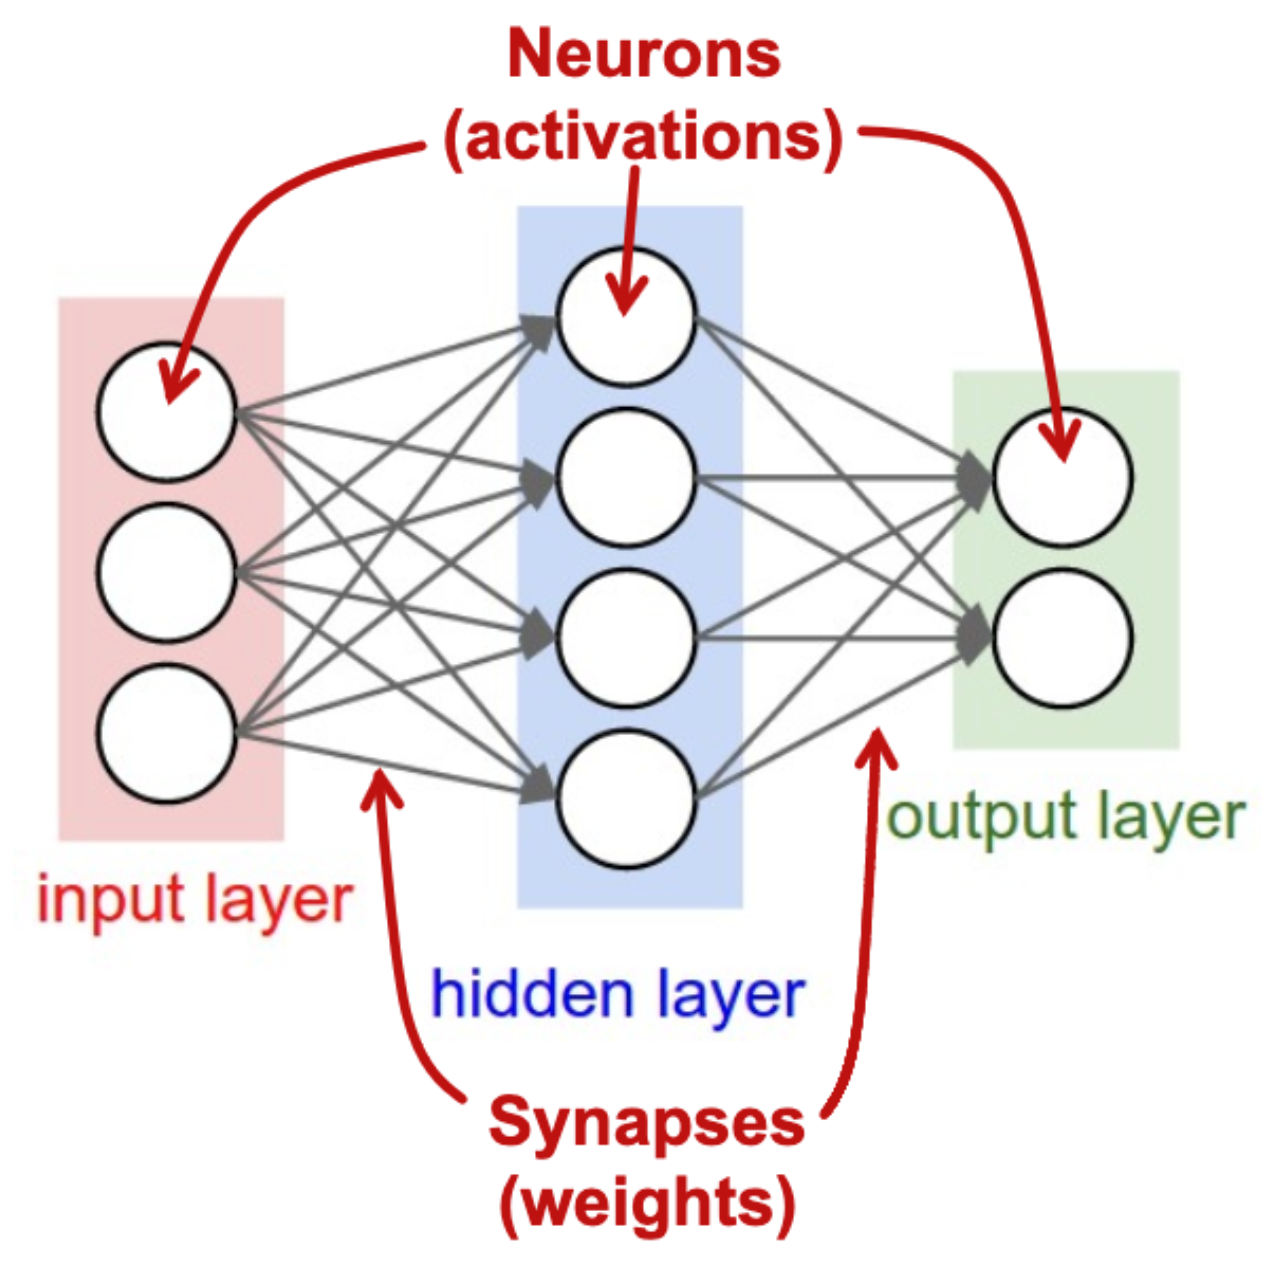
\includegraphics[width=0.4\textwidth]{ann}
    \caption[]{Structure of artificial feed-forward neural networks. Adopted from \citep{8114708}.}
    \label{fig:ann}
\end{figure}

The training of \acp{nn} is usually performed with the back-propagation algorithm which seeks to minimize a cost function $C(\bm{\varphi})$. This function measures the deviation of a presented input to a desired output dependent on the model parameters $\bm{\varphi}$. In deep a feed-forward \ac{nn} these model parameters are the mentioned weights and a bias term added to sum of the input weights per neuron. The minimum of this cost function can be found stepwise via gradient descent. Here, the update to the model parameters is guided by the negative of the gradient of the cost function, scaled by a learning rate $\gamma$
\begin{equation}
    \bm{\varphi}_{n+1} = \bm{\varphi}_n-\gamma\nabla C(\bm{\varphi}_n),
    \label{eq:grad_descent}
\end{equation}
such that moving against the gradient a monotonic decreasing series is formed $C(\bm{\varphi}_n )\ge C(\bm{\varphi}_{n+1})$ converging to a minimum of $C(\bm{\varphi})$. In three dimensions this is analogues to a mountaineer searching for the valley by going in the direction of the steepest descent with a stepsize proportional to $\gamma$.

\section{NEOS}
The central concept of \textit{\acl{neos}} involves employing a cost function that directly trains the \ac{ml} model with respect to the target quantity of interest. Insteaad of traditional classifier cost function that focuses only on differentiating between signal and background, the $\mathrm{CL}s$ value, detailed in Chapter \ref{sec:statistics}, is adopted as the quantity for minimization. For a typical analysis chain as shown in figure \ref{fig:neos} this translates into a mathematical concatenation of the individual steps within the chain.
\begin{figure}
    \centering
    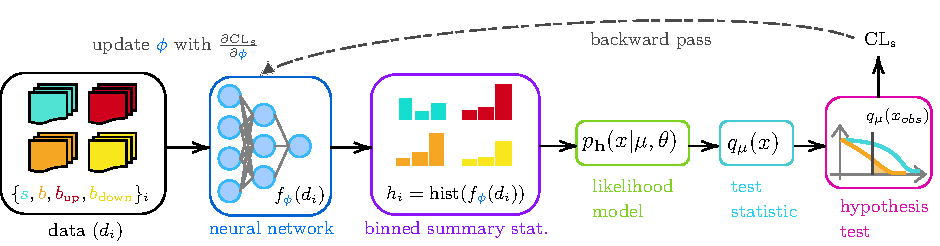
\includegraphics[width=1\textwidth]{neos}
    \caption[]{Typical particle physics analysis chain. For \ac{neos} the $\text{CL}_s$ value is back-propagated to train the neural network parameters $\bm{\varphi}$. Adopted from \citep{Simpson_2023}.}
    \label{fig:neos}
\end{figure}
Hence the cost function $\text{CL}_s$ is a function of the dataset $\mathcal{D}$ and the \ac{ml} model parameters $\bm{\varphi}$
\begin{equation}
    \mathrm{CL}_s = f(\mathcal{D},\bm{\varphi}) = (f_{\mathrm{sensitivity}} \circ f_{\mathrm{test\,stat}} \circ f_{\mathrm{likelihood}}  \circ f_{\mathrm{histogram}}  \circ f_{\mathrm{observable}})(\mathcal{D},\bm{\varphi}).
\end{equation}
In order to find the minimum via the gradient descent of equation \ref{eq:grad_descent} \cls needs to be differentiable with respect to $\bm{\varphi}$. By applying the chain rule this reads for one model parameter $\varphi_i$
\begin{equation}
    \frac{\partial\,\mathrm{CL}_s}{\partial \varphi_i} = \frac{\partial f_{\mathrm{sensitivity}}}{\partial f_{\mathrm{test\,stat}}}\frac{\partial f_{\mathrm{test\,stat}}}{\partial f_{ \mathrm{likelihood}}} \frac{\partial f_{\mathrm{likelihood}}}{\partial f_{\mathrm{histogram}}}   \frac{\partial f_{\mathrm{histogram}}}{\partial f_{\mathrm{observable}}}  \frac{\partial f_{\mathrm{observable}}}{\partial \varphi_i}.
\end{equation}
While all steps except histogramming are inherently differentiable, histogramming can be made differentiable through the application of \ac{kde}, as described by \citep{CRANMER2001198}. This technique involves approximating histograms by treating each data point as a normal distribution (kernel) centered at the data point value, with a bandwidth corresponding to the desired standard deviation. Since the area under each Gaussian is equal to one, the collective addition of all Gaussian's yields a smoothed estimate of a histogram that is inherently differentiable. However, it is crucial to select the bandwidth appropriately, ideally around the desired bin width, as the quality of the KDE estimate is sensitive to this choice. This is demonstrated in Figure \ref{fig:relaxed_hist}. Although this can be a source of uncertainty any differentiable step or block in figure \ref{fig:neos} can always be reverted and calculated exactly with the parameters found by the optimization.
\begin{figure}
    \centering
    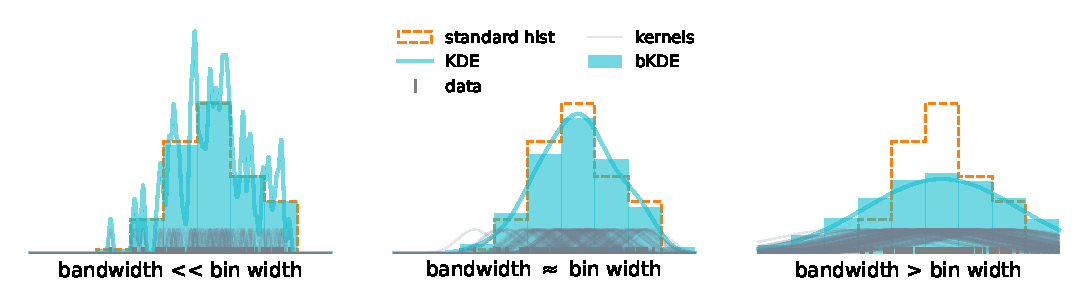
\includegraphics[width=1\textwidth]{relaxed_hist}
    \caption[]{Dependence of the histogram approximation with normal distributions of different standard deviations called bandwidth in the context of \ac{kde}. Depicted in grey small bars on the x-axis are the data points and in grey above them their kernel estimates. Further shown is the standard histogram binned from data, the \ac{kde} and the \ac{bkde} as a histogram calculated from the area under the \ac{kde} for some binning. Adopted from \citep{Simpson_2023}.}
    \label{fig:relaxed_hist}
\end{figure}


\section{Training}
In order to build the statistical model each histogram entering it needs to be created during training. This requires a full dataset per sample (signal, background estimate, some systematic, etc.) being processed through the whole pipeline. To make use of all available data and to avoid a training class imbalance bias each sample is upscaled by replicating values to the sample with the largest event content. Table \ref{tab:neos-samples} gives an overview of used samples in the training and the input variables per sample are shown in figure \ref{fig:tomats_inputs_0} and \ref{fig:tomats_inputs_1}. They are chosen from an impact ranking on a \mhh fit from fig. \red{fig reference}.


To ensure a fair training between features and to not let features with large values dominate the learning process a min-max scaling is applied to the input dataset
\begin{equation}
    x'=\frac{x - \text{min}(x)}{\text{max}(x)-\text{min}(x)}.
\end{equation}

\begin{table}[]
    \centering
    \caption{Samples and available number of events after the selection described in section \ref{hh4b_analysis_strategy} used in the training. Systematics are described in \ref{sec:systematics}. Deviations }
    \begin{tabular}{cc}
        \hline
        Sample                                                                                         & Events \\ \hline 
        Data Background Estimate                                                                       & 21913   \\ \hline
        VBF Signal $\kappa_\mathrm{2V}=0$ Nominal                                                      & 43492  \\
        VBF Signal $\kappa_\mathrm{2V}=0$ systematic: GN2X pt bin 0 up                                 & 43492  \\
        VBF Signal $\kappa_\mathrm{2V}=0$ systematic: GN2X pt bin 0 down                               & 43492  \\
        VBF Signal $\kappa_\mathrm{2V}=0$ systematic: GN2X pt bin 1 up                                 & 43492  \\
        VBF Signal $\kappa_\mathrm{2V}=0$ systematic: GN2X pt bin 1 down                               & 43492  \\
        VBF Signal $\kappa_\mathrm{2V}=0$ systematic: GN2X pt bin 2 up                                 & 43492  \\
        VBF Signal $\kappa_\mathrm{2V}=0$ systematic: GN2X pt bin 2 down                               & 43492  \\
        VBF Signal $\kappa_\mathrm{2V}=0$ systematic: GN2X pt bin 3 up                                 & 43492  \\
        VBF Signal $\kappa_\mathrm{2V}=0$ systematic: GN2X pt bin 3 down                               & 43492  \\
        VBF Signal $\kappa_\mathrm{2V}=0$ systematic: JET EtaIntercalibration NonClosure PreRec up     & 44126  \\
        VBF Signal $\kappa_\mathrm{2V}=0$ systematic: JET EtaIntercalibration NonClosure PreRec down   & 42737  \\
        VBF Signal $\kappa_\mathrm{2V}=0$ systematic: JET EtaIntercalibration Modelling up             & 43917  \\
        VBF Signal $\kappa_\mathrm{2V}=0$ systematic: JET EtaIntercalibration Modelling down           & 42984  \\
        VBF Signal $\kappa_\mathrm{2V}=0$ systematic: Scale Variation $\mu_R = 0.5, \mu_F=0.5$         & 43492  \\
        VBF Signal $\kappa_\mathrm{2V}=0$ systematic: Scale Variation $\mu_R = 0.5, \mu_F=1.0$         & 43492  \\
        VBF Signal $\kappa_\mathrm{2V}=0$ systematic: Scale Variation $\mu_R = 1.0, \mu_F=0.5$         & 43492  \\
        VBF Signal $\kappa_\mathrm{2V}=0$ systematic: Scale Variation $\mu_R = 1.0, \mu_F=1.0$         & 43492  \\
        VBF Signal $\kappa_\mathrm{2V}=0$ systematic: Scale Variation $\mu_R = 1.0, \mu_F=2.0$         & 43492  \\
        VBF Signal $\kappa_\mathrm{2V}=0$ systematic: Scale Variation $\mu_R = 2.0, \mu_F=1.0$         & 43492  \\
        VBF Signal $\kappa_\mathrm{2V}=0$ systematic:         Scale Variation $\mu_R = 2.0, \mu_F=2.0$ & 43492  \\ \hline
        VBF Signal $\kappa_\mathrm{2V}=0$ \ac{cr} GN2X tags: 1                                         & 142443 \\
        VBF Signal $\kappa_\mathrm{2V}=0$ \ac{cr} GN2X tags: 2                                         & 544    \\
        VBF Signal $\kappa_\mathrm{2V}=0$ \ac{vr} GN2X tags: 1                                         & 57098  \\
        VBF Signal $\kappa_\mathrm{2V}=0$ \ac{vr} GN2X tags: 2                                         & 243    \\
    \end{tabular}
    \label{tab:neos-samples}
\end{table}


\begin{figure}
    \centering
    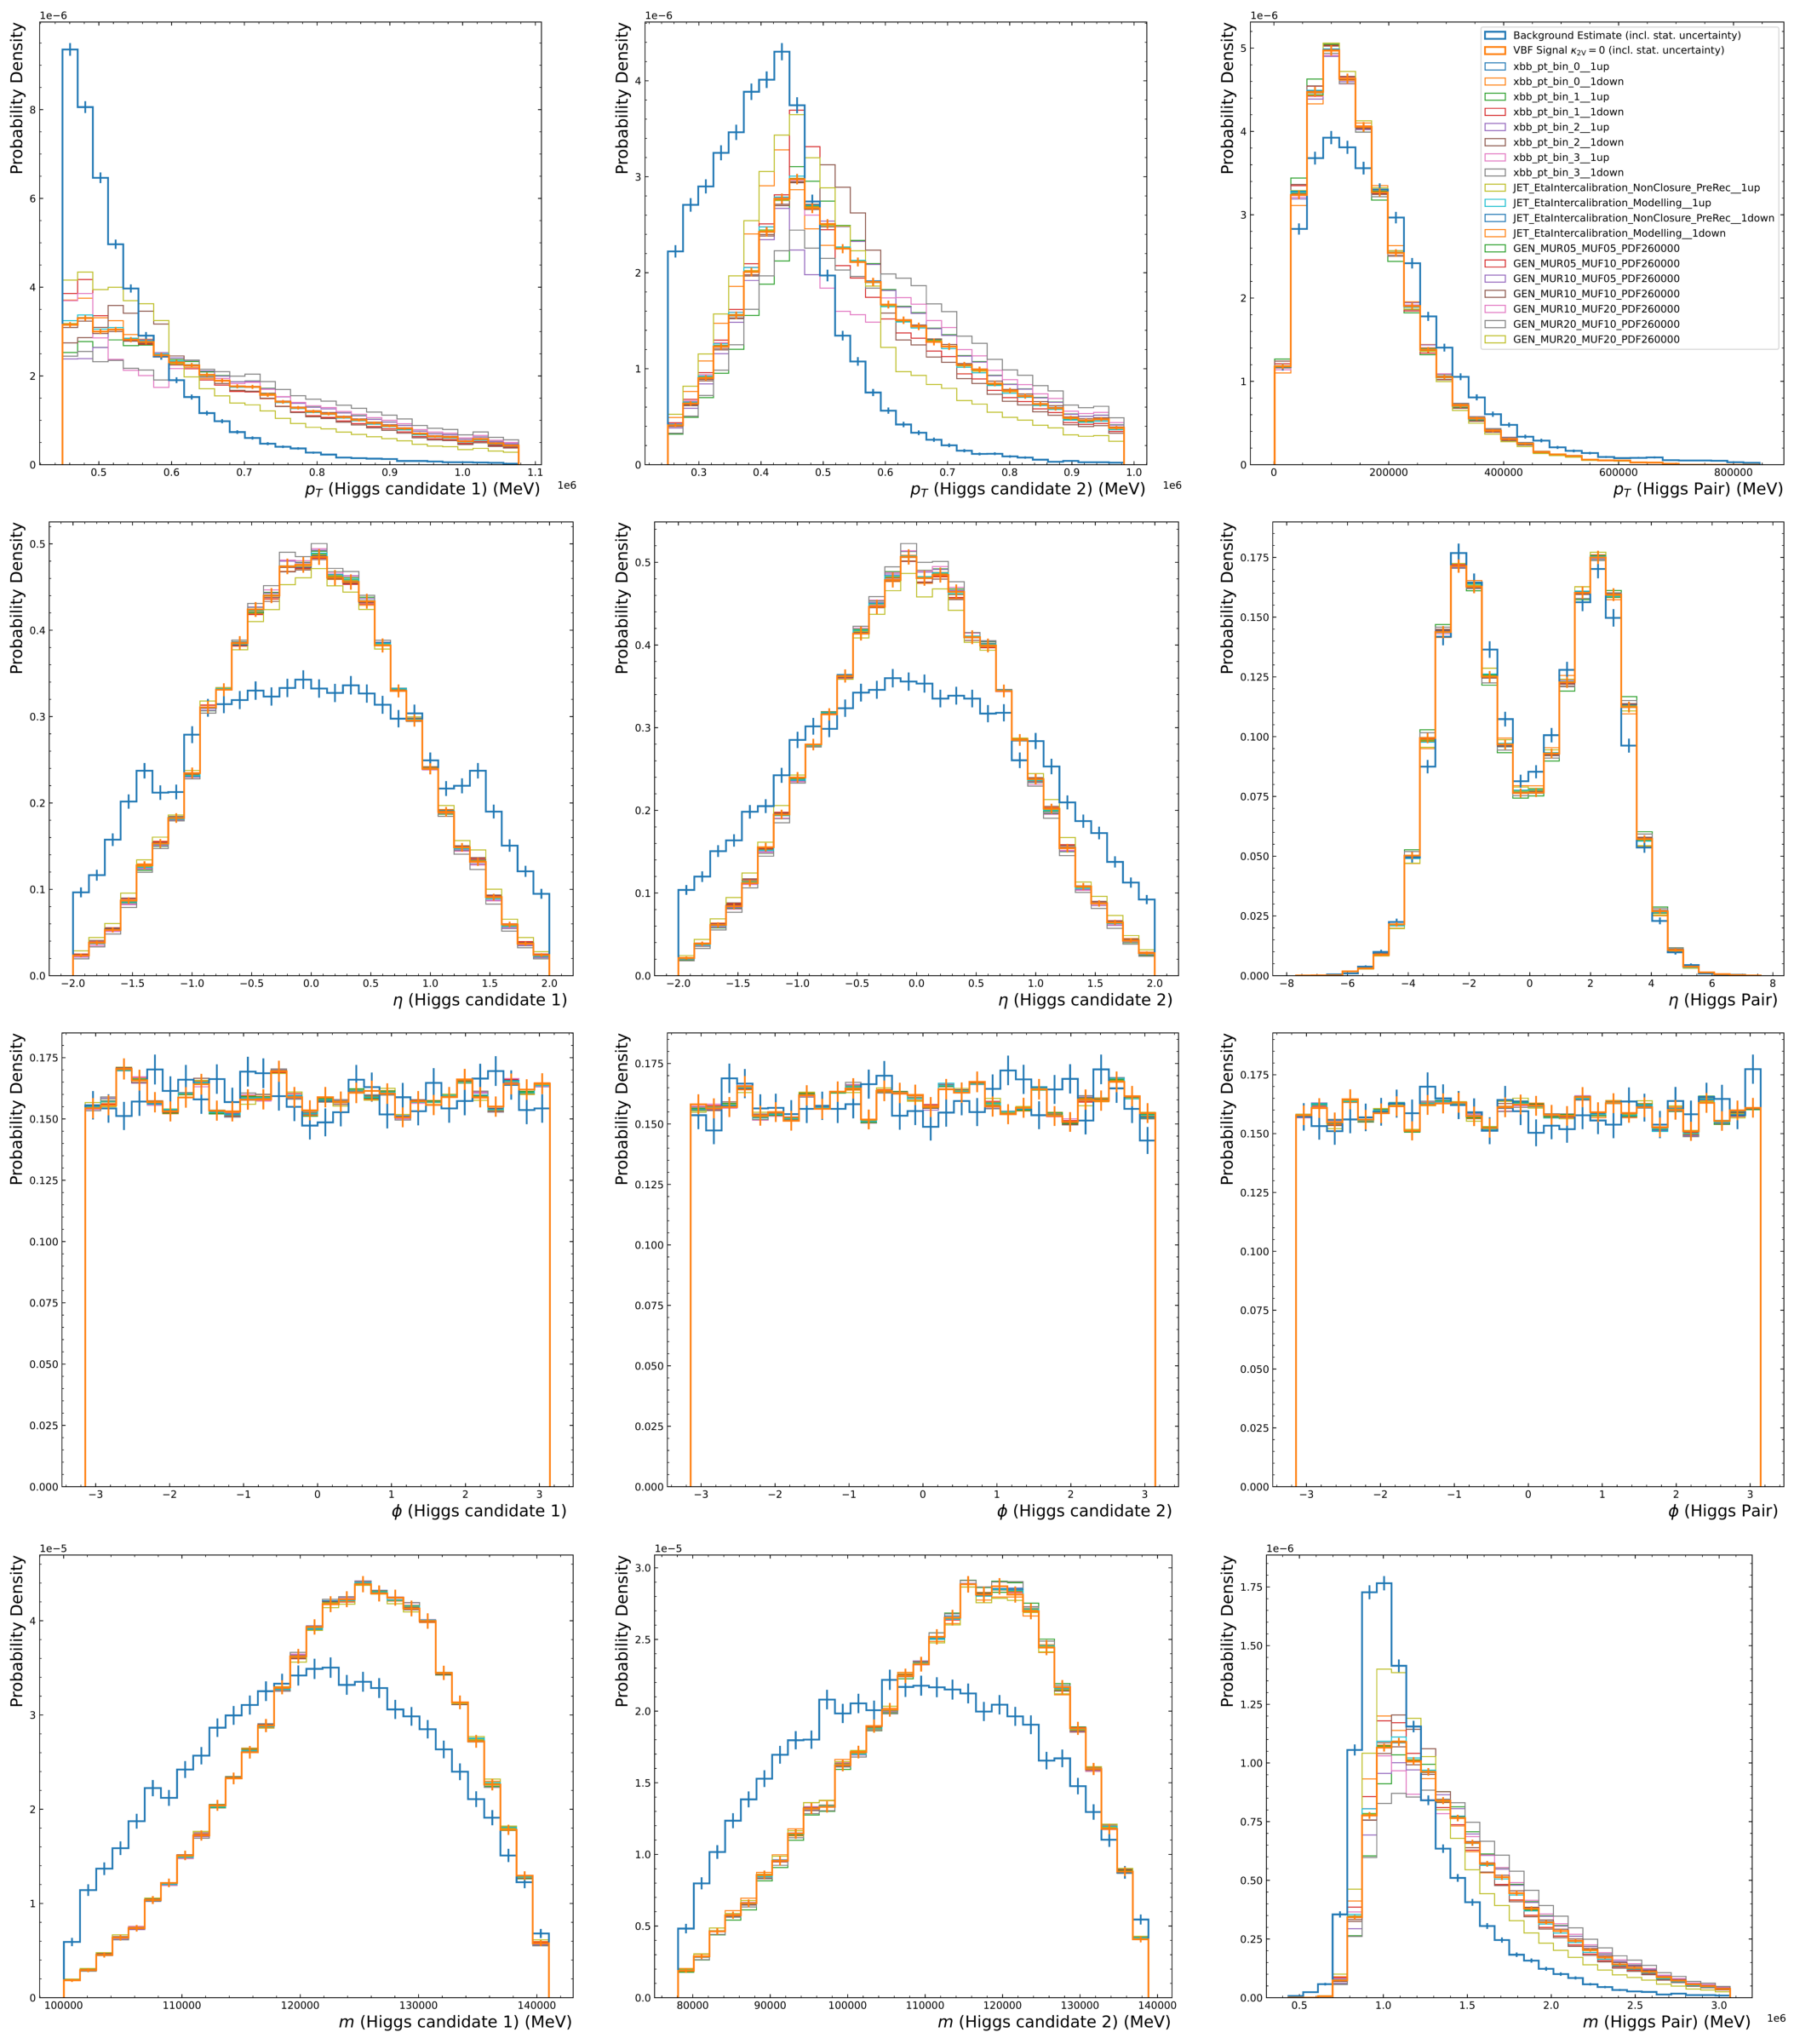
\includegraphics[width=1\textwidth]{tomats_inputs_0}
        \caption[]{Neos input variables (1/2)}
    \label{fig:tomats_inputs_0}    
\end{figure}



\begin{figure}
    \centering
    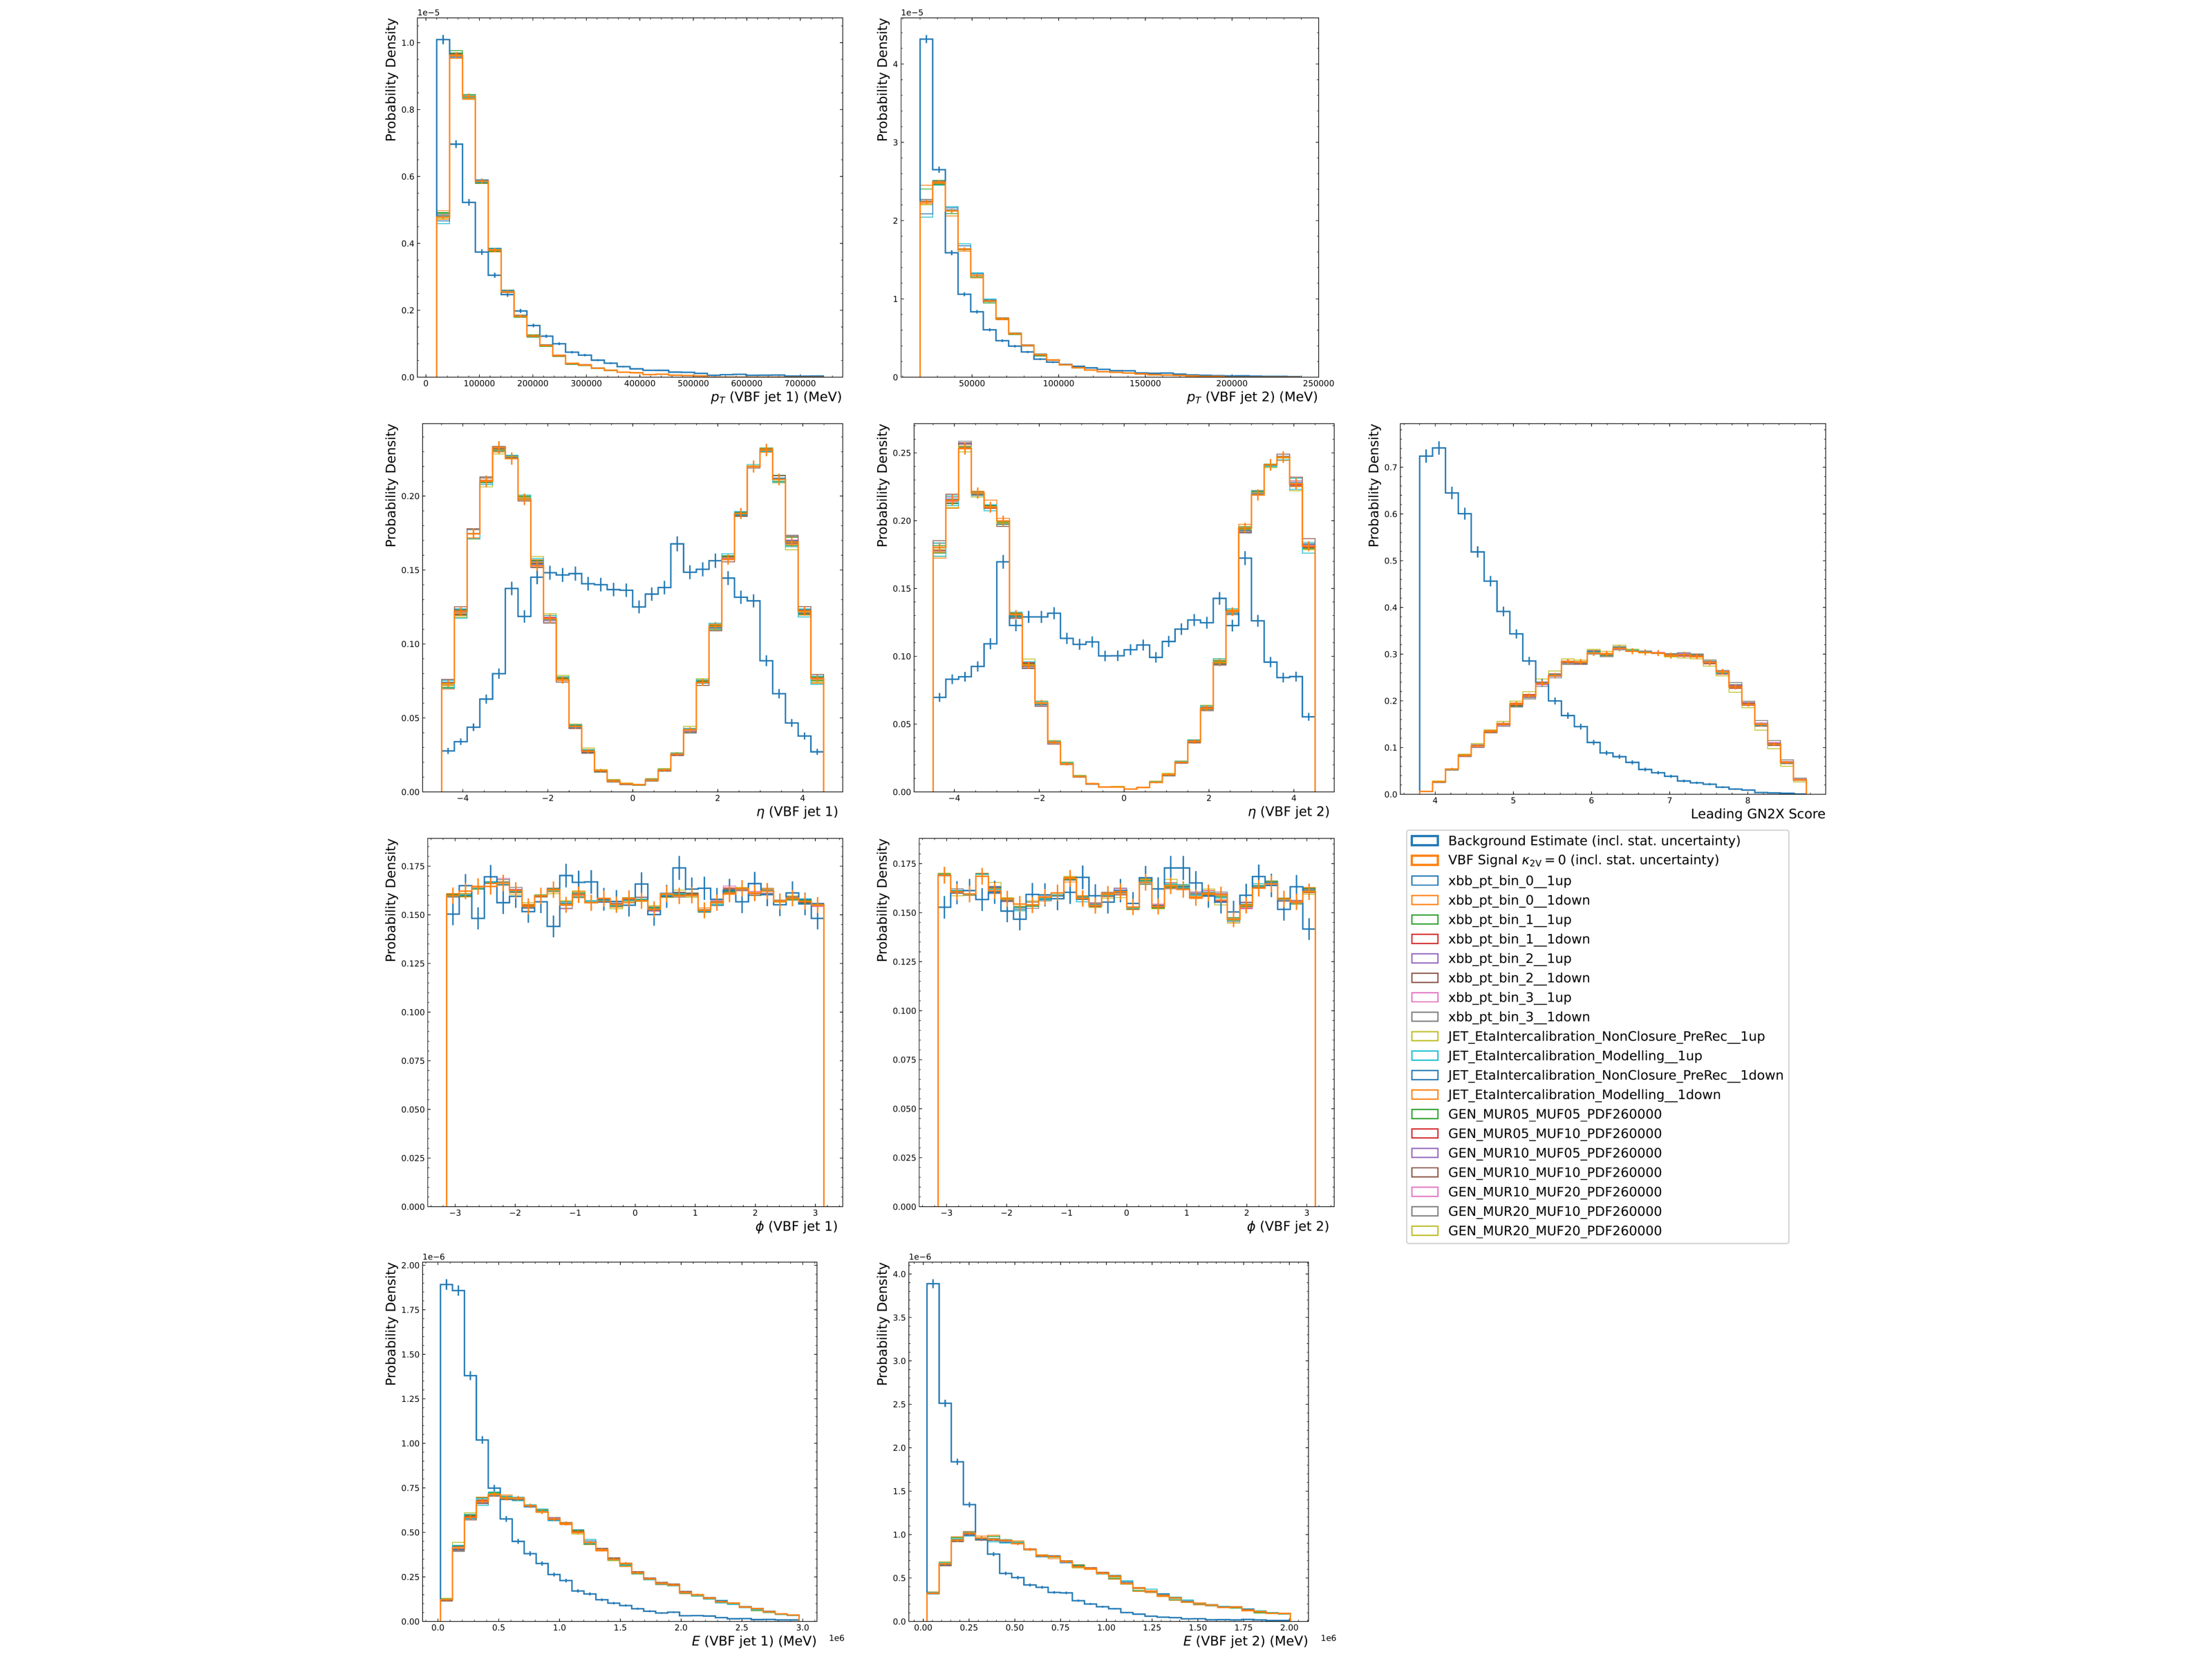
\includegraphics[width=1\textwidth]{tomats_inputs_1}
        \caption[]{Neos input variables (2/2)}
    \label{fig:tomats_inputs_1}    
\end{figure}





% preprocess
min max scaled

run2 sr_xbb1
22111
k2v0 sr_xbb2
NOSYS
43518
JET_EtaIntercalibration_NonClosure_PreRec__1up
44152

bkg upscaled with a factor of ~2


everythign is upscaled to the largest array
JET_EtaIntercalibration_NonClosure_PreRec__1up


in order for the batching mechanism to work
signal samples upscaled due to slight variations in the selection caused by some systematic uncertainty the largest sample size


send each systematics dataset through nn

#train test split

% _m_jj_eta_jj does not help during training, maybe only if cuts are offf????

% 5 bins 
% self.vars = [
%     "pt_j1",
%     "eta_j1",
%     "phi_j1",
%     "E_j1",
%     "pt_j2",
%     "eta_j2",
%     "phi_j2",
%     "E_j2",
%     "pt_h1",
%     "eta_h1",
%     "phi_h1",
%     "m_h1",
%     "pt_h2",
%     "eta_h2",
%     "phi_h2",
%     "m_h2",
%     "pt_hh",
%     "eta_hh",
%     "phi_hh",
%     "m_hh",
%     "lead_xbb_score",
%     "m_jj",
%     "eta_jj",
% ]
% self.systematics = [
%     "NOSYS",
%     "xbb_pt_bin_0__1up",
%     "xbb_pt_bin_0__1down",
%     "xbb_pt_bin_1__1up",
%     "xbb_pt_bin_1__1down",
%     "xbb_pt_bin_2__1up",
%     "xbb_pt_bin_2__1down",
%     "xbb_pt_bin_3__1up",
%     "xbb_pt_bin_3__1down",
%     "JET_EtaIntercalibration_NonClosure_PreRec__1up",
%     "JET_EtaIntercalibration_Modelling__1up",
%     "JET_EtaIntercalibration_NonClosure_PreRec__1down",
%     "JET_EtaIntercalibration_Modelling__1down",
%     "GEN_MUR05_MUF05_PDF260000",
%     "GEN_MUR05_MUF10_PDF260000",
%     "GEN_MUR10_MUF05_PDF260000",
%     "GEN_MUR10_MUF10_PDF260000",
%     "GEN_MUR10_MUF20_PDF260000",
%     "GEN_MUR20_MUF10_PDF260000",
%     "GEN_MUR20_MUF20_PDF260000",
%     stat error
% ]

\red{is saved and loaded in selection}

\section{Performance}
\red{in results part}

\subsection{Implementation}
Tracing differentiation through software is achievable by recognizing that any software essentially comprises a series of elementary arithmetic operations. Since the analytic solutions for these operations are known, the task reduces to concatenating all these operations and differentiating the resulting function. This is also known as \textit{Automatic Differentiation} and is achieved here with the help of the software package \textsc{jax} \citep{jax2018github}.

While the concept may appear straightforward, one of the challenges that previously hindered its implementation is the difficulty of differentiating across multiple individual software frameworks.That this became feasible within a reasonable time frame builds greatly on the transition efforts  of the individual steps to the \textsc{Python} programming language, moving away from C++ \textsc{ROOT}-based software \citep{ANTCHEVA20092499}. While \textsc{root} was indispensable at its time of emergence it is now less optimal for contemporary scientific analysis. This is because it is not only more difficult to integrate within other current software but also due to its user-unfriendliness compared to \textsc{Python} solutions which are maintained by a broad scientific community doing data-analysis. Using \textsc{python} in this context presents a notable advantage since it benefits from widespread community support and pre-existing solutions to many common problems, enabling the use of tools like \textsc{jax}, which are not originally connected to \ac{hep}.

The original proposers \citet{Simpson_2023} of \ac{neos} developed differentiable versions of common \ac{hep} tasks like the upper mentioned hypothesis test, histogramming and the optimization of a cut in a packaged called \textsc{relaxed} \citep{Simpson_relaxed_version_0_3_0_2023}. They successfully tested the entire pipeline in a toy model \citep{Simpson_neos_version_0_2_0_2021}. These efforts were transferred and further developed to be applicable to this analysis with \citep{hh_neos}.


\red{ this somewhere here, or outlook?
    stack several neural networks together!!! end to end training
    one for pairing, event selection
    stack arbitrarily
    selling point ist binning ist optimiert, auch mit fixen bins
}

\red{
    welche unsicherheiten wurden für training benutzt
    tight starting condition, also stabilizes/increase training convergence, but local minimum?
    optimization turns cuts off entirely
}